\section{Trigger and Reconstruction Bias}

We determine the size of this systematic uncertainty using a leading-order
Monte Carlo evaluation of $A_{LL}$. We start with the kinematics and hard
scattering subprocess of each Pythia event and determine numerator and
denominator weights by calculating a partonic $a_{LL}$ and sampling from
polarized and unpolarized parton distribution functions. We can use these
weights to calculate an $A_{LL}$ for any set of simulated events.
Specifically, we can measure the difference between the ``true'' $A_{LL}$ for
all Pythia events and the ``reconstructed'' $A_{LL}$ using only triggered
events with reconstructed charged pions and use that to assign the systematic
uncertainty.

This procedure obviously requires that our Monte Carlo generator does a good
job of reproducing the actual event kinematics. Unfortunately, we have found
that the fragmentation tune in Pythia 6.4 is not quite up to the task. In
Figure \ref{fig:subprocess-fractions} we compare the subprocess contributions
to charged pion production reported by Pythia with the results of NLO pQCD
calculations incorporating Kretzer and DSS fragmentation functions. The DSS
set is known to better describe RHIC kinematics, but in Figure
\ref{fig:subprocess-fractions} it's clear that Pythia agrees much better with
Kretzer.

\begin{figure}
  \subfigure[Kretzer]{
    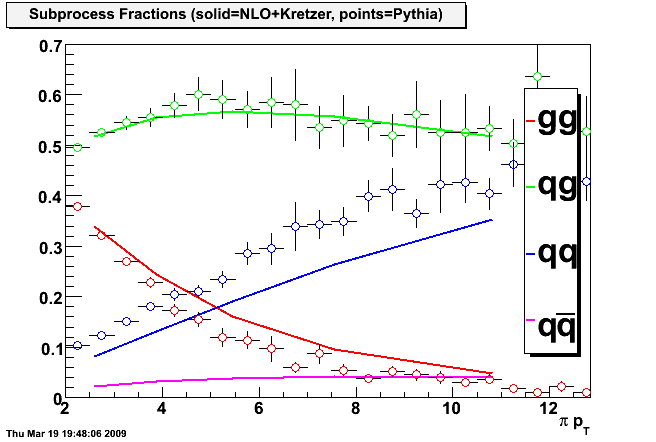
\includegraphics[width=0.5\textwidth]{figures/pythia-kretzer}
    \label{fig:pythia-kretzer}
  }
  \subfigure[DSS]{
    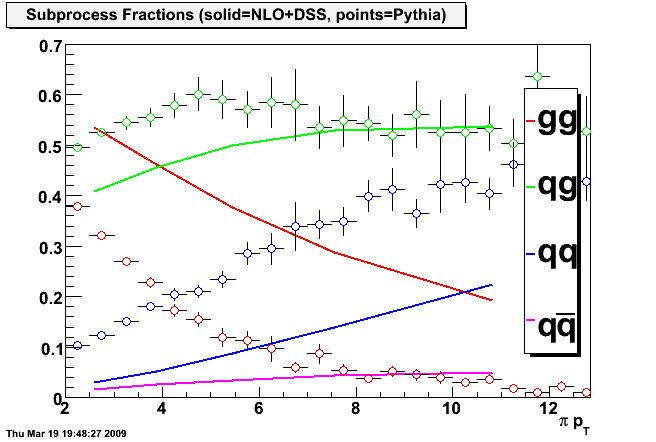
\includegraphics[width=0.5\textwidth]{figures/pythia-dss}
    \label{fig:pythia-dss}
  }
  \caption{Comparison of subprocess contributions to charged pion production
  in Pythia and NLO pQCD calculations incorporating two different
  fragmentation functions. The Pythia results agree much better with the
  calculations using Kretzer fragmentation functions}
  \label{fig:subprocess-fractions}
\end{figure}

Getting the subprocess contributions right is an important precondition for
using the Method of Asymmetry Weights to evaluate trigger and reconstruction
bias, quite simply because $A_{LL}$ has such a strong subprocess dependence.
To confirm that the problem is really isolated to Pythia's fragmentation
functions, we examined the ratio of pions fragmenting from the quark and the
gluon in qg scattering events. That ratio is shown in Figure
\ref{fig:qg-fragmentation}, and confirms that the fragmentation model is
Kretzer-like, with much softer gluon fragmentation and/or harder quark
fragmentation than we observe at RHIC.

\begin{figure}
  \begin{center}
    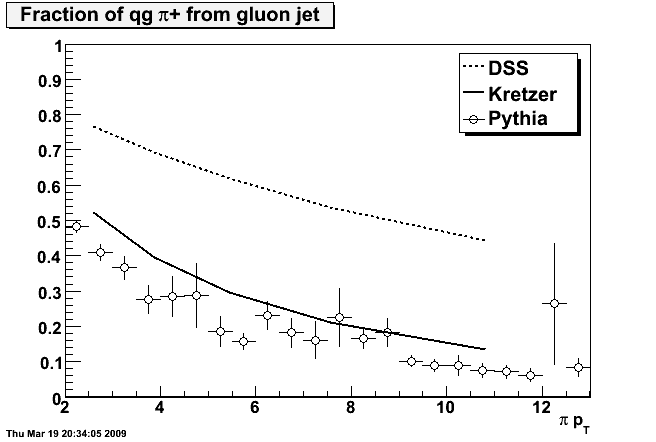
\includegraphics[width=0.7\textwidth]{figures/qg-fragmentation}
  \end{center}
  \caption{Fraction of pions produced in quark-gluon scattering events that
  fragment from the gluon. Once again, the Pythia distributions agree much
  better with the calculation that uses Kretzer fragmentation functions.}
  \label{fig:qg-fragmentation}
\end{figure}

We decided that, rather than plumb the depths of Pythia's independent
fragmentation model, we would apply a $p_{T}$- and subprocess-dependent
reweighting factor to our simulations to generate DSS-like fragmentation. The
effect of this reweighting is shown in Figure \ref{fig:compare-mcasym-nlo}.
The filled markers show markedly better agreement with the NLO pQCD
calculations than the open markers, particularly in scenarios such as GRSV-MIN
where the difference in $A_{LL}$ between gg and qg subprocesses is large. The
agreement is still not perfect; one might speculate that Pythia gives too much
weight to favored quark fragmentation, since at high $p_{T}$ the $\pi^{-}$
asymmetries are too small (indicating a relatively large d quark contribution)
and the $\pi^{+}$ asymmetries are too large (consistent with a large u quark
contribution). However, as the trigger and reconstruction is not expected to
be quark flavor dependent we have decided to press forward with these
simulations.

\begin{figure}
  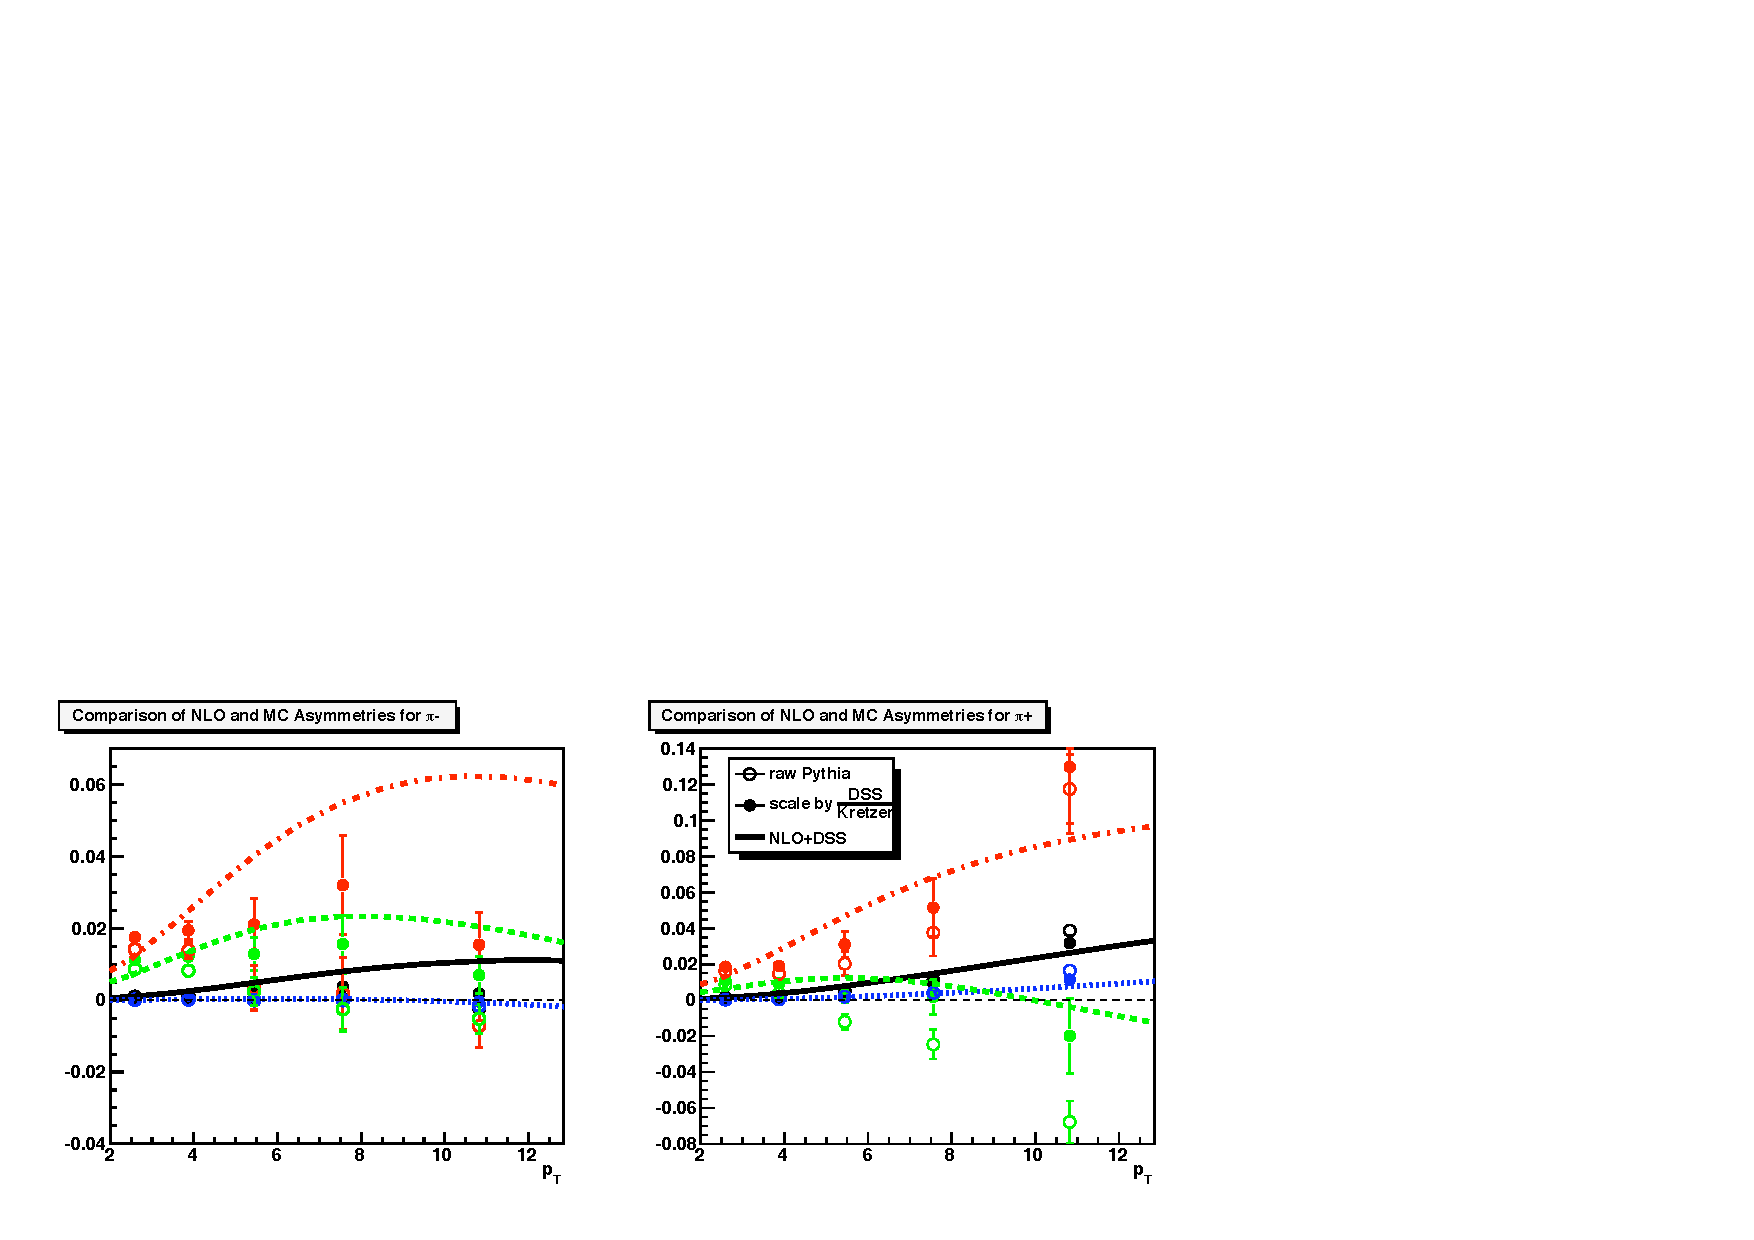
\includegraphics[width=\textwidth]{figures/compare-mcasym-nlo}
  \caption{Comparison of Monte Carlo asymmetries with NLO pQCD calculations
  incorporating DSS fragmentation functions. The open markers show results
  obtained using STAR's Pythia tune. The filled markers show the change in the
  asymmetries after reweighting the gg, qg, and qq distributions by the ratio
  of subprocess fractions calculated using DSS and Kretzer fragmentation
  functions.}
  \label{fig:compare-mcasym-nlo}
\end{figure}

Figure \ref{fig:mcasym-diff} examines the difference between asymmetries for a
``true'' sample using untriggered events and pions pulled straight from the
Pythia record, and a ``trigger+reco'' sample where the events must satisfy the
JP2 trigger simulator and the pion kinematics are obtained from TPC track
reconstruction. In some cases, the difference between the two samples is
smaller than the uncertainty on the ``trigger+reco'' sample (see Figure
\ref{fig:mcasym-sigma}). We use the larger of the two to assign the
systematic.

The size of the systematic obviously depends on the polarized gluon
distributions that are included in the analysis. Previous measurements have
excluded the maximal polarization scenarios as well as scenarios with the
functional form of the GRSV set and integral gluon polarizations larger than
STD. As a result, we use an envelope defined by the GRSV M105 and STD
scenarios. The results of this analysis are shown in Table
\ref{tbl:trig-reco-bias}.

\begin{figure}
  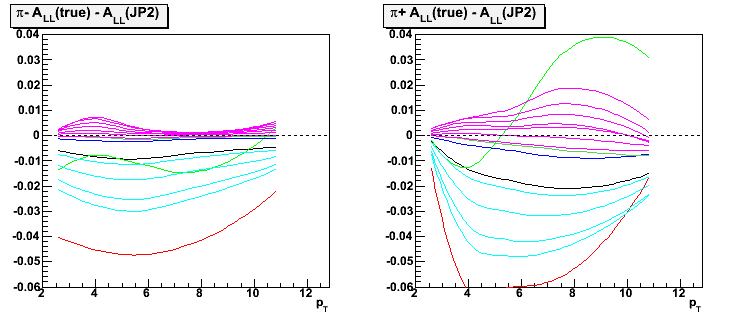
\includegraphics[width=\textwidth]{figures/mcasym_run5_diff_rescaled}
  \caption{Difference between true and reconstructed Monte Carlo
  asymmetries after fragmentation reweighting.}
  \label{fig:mcasym-diff}
\end{figure}

\begin{figure}
  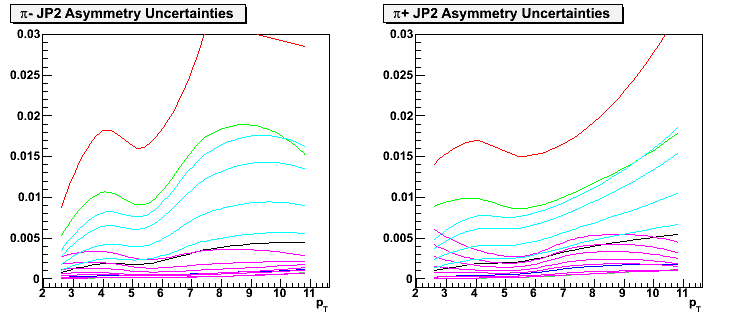
\includegraphics[width=\textwidth]{figures/mcasym_run5_sigma_rescaled}
  \caption{Uncertainty on reconstructed Monte Carlo asymmetries. If the
  uncertainty is larger than the difference between true and reconstructed
  asymmetries we use this to assign the systematic instead.}
  \label{fig:mcasym-sigma}
\end{figure}

\begin{table}[ht]
    \begin{center}
        \begin{tabular}{c|c|c}
        \hline
        $p_{T}$ bin & $\pi^{-}$ uncertainty & $\pi^{+}$ uncertainty\\
        \hline
        \hline
        [2.00 - 3.18] & -0.0059 +0.0027 & -0.0061 +0.0061\\
        \hline
        [3.18 - 4.56] & -0.0083 +0.0072 & -0.0128 +0.0066\\
        \hline
        [4.56 - 6.32] & -0.0093 +0.0034 & -0.0176 +0.0101\\
        \hline
        [6.32 - 8.80] & -0.0072 +0.0036 & -0.0209 +0.0186\\
        \hline
        [8.80 - 12.84] & -0.0048 +0.0057 & -0.0152 +0.0062\\
    \hline
    \end{tabular}
    \end{center}
    \caption{Trigger and Reconstruction Bias Uncertainties}
    \label{tbl:trig-reco-bias}
\end{table}
